% !TeX program = lualatex
% ================================================================
% Polish Parallel Text Version of InequalitiesRevision
%
% Generated by the server using the following settings:
%
%   language            Polish (pol)
%   text direction      left to right
%   font                Noto Serif
%   fallback font       Noto Serif
%   built from          latex/worksheets/revision/inequalitiesRevision.tex
%   vocabulary key      latex/worksheets/revision/inequalitiesRevision/L2/pol/inequalitiesRevision_polishKey.tex
%   tier 3 vocabulary   green   RGB 0 128 0
%   English text        black   RGB 0 0 0
%   Polish text         purple  RGB 112 48 160
%   layout macros       version 3
%
% Please don't edit any information in this comment block - the server
% compares it against the current settings and rebuilds this file when
% they differ, so changes here would be overwritten. However, feel free
% to make updates to the LaTeX below if you want to edit it.
% ================================================================

\documentclass[11pt,a4paper]{article}
% ================================================================
% Copied from the English sheet this was translated from, so that
% anything it sets up for itself still works here
% ================================================================
\usepackage[a4paper,top=14mm,bottom=14mm,left=15mm,right=15mm]{geometry}
\usepackage[T1]{fontenc}
\usepackage{amsmath}
\usepackage{amssymb}
\usepackage{array}
\usepackage{multicol}
\usepackage{tikz}
\usetikzlibrary{arrows.meta}

% ================================================================
% Inequalities: revision questions.
%
% Two pages of questions, in black and white, with a heading for each
% topic on the Maths Revision topic list in the same order. Each topic
% has a few short questions that start easy, with a diagram only where
% a question uses one, and the sheet ends with some problem solving.
% There are no key facts or worked examples on the sheet: the methods
% are in the worked solutions and the revision guide. Questions are
% numbered through the sheet so that the answer key and the worked
% solutions can refer to them.
% ================================================================

\pagestyle{empty}
\setlength{\parindent}{0pt}
\setlength{\parskip}{2pt}
\setlength{\columnsep}{9mm}

% A topic from the revision list.
\newcommand{\topic}[1]{\par\addvspace{14pt}{\bfseries #1}\par\nobreak\vspace{2pt}}

% Questions are numbered through the whole sheet.
\newcounter{qn}
\newcommand{\q}{\par\addvspace{9pt}\stepcounter{qn}\hangindent=1.6em\hangafter=1\noindent
  \makebox[1.6em][l]{\textbf{\theqn}}}

% \numline{<label>}{<drawing>}: a number line from -4 to 5, with the
% drawing placed at height 4, above the line.
\newcommand{\numline}[2]{%
  \begin{tikzpicture}[x=6.5mm,y=1mm]
    \node[anchor=east] at (-4.9,0) {#1};
    \draw[{Stealth[length=1.5mm]}-{Stealth[length=1.5mm]}] (-4.6,0) -- (5.6,0);
    \foreach \n in {-4,...,5}{\draw (\n,-1) -- (\n,1); \node[below,font=\small] at (\n,-1) {$\n$};}
    #2
  \end{tikzpicture}}
\newcommand{\opencircle}[1]{\draw[thick,fill=white] (#1,4) circle (1.2mm);}
\newcommand{\filledcircle}[1]{\fill (#1,4) circle (1.2mm);}

% \smallgraph{<shading>}{<boundary line>}: axes from -2 to 4. The grid is
% drawn over the shading, and the boundary line over the grid.
\newcommand{\smallgraph}[2]{%
  \begin{tikzpicture}[x=4.6mm,y=4.6mm,font=\scriptsize]
    #1
    \draw[black!25,step={(1,1)}] (-2,-2) grid (4,4);
    #2
    \draw[-{Stealth[length=1mm]}] (-2,0) -- (4.5,0) node[right] {$x$};
    \draw[-{Stealth[length=1mm]}] (0,-2) -- (0,4.5) node[above] {$y$};
    \foreach \t in {2,4}{\node[below] at (\t,0) {\t}; \node[left] at (0,\t) {\t};}
  \end{tikzpicture}}

% Characters this language's font has not got are borrowed from another,
% rather than being silently dropped - see docs/translated-sheet-latex.md
\directlua{%
  if luaotfload and luaotfload.add_fallback then
    luaotfload.add_fallback("eallatinfallback",
      { "Noto Serif:mode=harf;" })
  else
    tex.error("this luaotfload is too old to register a fallback font")
  end
}
\usepackage[english]{babel}
\babelprovide[import]{polish}
\babelfont[polish]{rm}[Renderer=Harfbuzz, BoldFont={Noto Serif}, ItalicFont={Noto Serif}, BoldItalicFont={Noto Serif}, RawFeature={fallback=eallatinfallback}]{Noto Serif}
\babelfont[polish]{sf}[Renderer=Harfbuzz, BoldFont={Noto Serif}, ItalicFont={Noto Serif}, BoldItalicFont={Noto Serif}, RawFeature={fallback=eallatinfallback}]{Noto Serif}
\newcommand{\ealtext}[1]{\foreignlanguage{polish}{#1}}
\newcommand{\ealtextblock}[1]{{\raggedright\foreignlanguage{polish}{#1}\par}}
% ================================================================
% EAL layout helpers
% ================================================================
\usepackage{xcolor}

\definecolor{ealkeycolour}{RGB}{0,128,0}
\definecolor{ealenglish}{RGB}{0,0,0}
\definecolor{ealtwocolour}{RGB}{112,48,160}

\newsavebox{\ealboxen}
\newsavebox{\ealboxtr}
\newlength{\ealglosswd}
\newlength{\ealglossraise}
\setlength{\ealglossraise}{1.15em}

% a tier 3 word, in English and in translation alike
\newcommand{\ealkey}[1]{\textcolor{ealkeycolour}{#1}}
\newcommand{\ealkeytr}[1]{\textcolor{ealkeycolour}{\ealtext{#1}}}

% One translated word above one English word. Built from kernel
% primitives, never a tabular, which would break wherever the sheet
% loads array, booktabs or tabularx. The box is as wide as the wider of
% the two, so a long translation pushes its neighbours aside instead of
% overlapping them, and it claims its full height so a table row or a
% TikZ node makes room for it.
\newcommand{\ealgloss}[2]{%
  \sbox{\ealboxen}{\ealkey{#1}}%
  \sbox{\ealboxtr}{\small\textcolor{ealtwocolour}{\ealtext{#2}}}%
  \setlength{\ealglosswd}{\wd\ealboxen}%
  \ifdim\wd\ealboxtr>\ealglosswd\setlength{\ealglosswd}{\wd\ealboxtr}\fi
  \leavevmode
  \makebox[\ealglosswd][c]{%
    \makebox[0pt][c]{\usebox{\ealboxen}}%
    \makebox[0pt][c]{\raisebox{\ealglossraise}{\usebox{\ealboxtr}}}%
  }%
}

% opens up line spacing around a block of glosses, so the raised
% translations sit clear of the line above
\newenvironment{ealglossed}{\par\linespread{2.1}\selectfont\ignorespaces}{\par}

% a whole translated sentence above its English counterpart. block level,
% so it does not belong inside a tabular cell
\newcommand{\ealpara}[2]{%
  \par\addvspace{0.5\baselineskip}%
  {\color{ealtwocolour}\ealtextblock{#1}}%
  \penalty200
  {\color{ealenglish}#2\par}%
  \addvspace{0.5\baselineskip}%
}

\begin{document}
% Ragged right, without \raggedright, which would make \\ end the
% paragraph and lose the hanging indent of a question's later lines.
\setlength{\rightskip}{0pt plus 4em}

\ealpara{\Large\bfseries \ealkeytr{Nierówności}\hfill{\large Pytania powtórkowe}}{\Large\bfseries \ealkey{Inequalities}\hfill{\large Revision questions}}
\par\vspace{2pt}\hrule\vspace{4pt}

\begin{multicols}{2}

% ----------------------------------------------------------------
\ealpara{Czytanie i rysowanie \ealkeytr{nierówności} na \ealkeytr{osiach liczbowych}}{\topic{Reading and drawing \ealkey{inequalities} on \ealkey{number lines}}}
\ealpara{Zapisz \ealkeytr{nierówność} pokazaną na każdej \ealkeytr{osi liczbowej}}{\q Write down the \ealkey{inequality} shown on each \ealkey{number line}.\\[4pt]
\numline{(a)}{\draw[very thick,-{Stealth[length=1.8mm]}] (1,4) -- (5.6,4); \opencircle{1}}\\[5pt]
\numline{(b)}{\draw[very thick,-{Stealth[length=1.8mm]}] (-2,4) -- (-4.6,4); \filledcircle{-2}}\\[5pt]
\numline{(c)}{\draw[very thick] (-3,4) -- (2,4); \filledcircle{-3} \opencircle{2}}}
\ealpara{Pokaż każdą \ealkeytr{nierówność} na \ealkeytr{osi liczbowej}}{\q Show each \ealkey{inequality} on a \ealkey{number line}.\\
(a) $x\ge4$\qquad (b) $-1<x\le5$}
\ealpara{Wypisz \ealkeytr{liczby całkowite}, które \ealkeytr{spełniają}}{\q List the \ealkey{integers} that \ealkey{satisfy}\\
(a) $-1<x\le5$\qquad (b) $-5<x<-1$}
\ealpara{Temperatura wewnątrz lodówki, $t\,^\circ$C, musi wynosić co najmniej 1\,$^\circ$C i mniej niż 5\,$^\circ$C. Zapisz to jako \ealkeytr{nierówność} i pokaż ją na \ealkeytr{osi liczbowej}.}{\q The temperature inside a fridge, $t\,^\circ$C, must be at least 1\,$^\circ$C and less than 5\,$^\circ$C. Write this as an \ealkey{inequality}, and show it on a \ealkey{number line}.}

% ----------------------------------------------------------------
\ealpara{Jak \ealkeytr{rozwiązać} \ealkeytr{nierówności}}{\topic{\ealkey{Solving} \ealkey{inequalities}}}
\ealpara{\ealkeytr{Rozwiąż}\quad (a) $x+7>12$\qquad (b) $4x\le28$\\[3pt]
(c) $2x-3<11$\qquad (d) $\dfrac{x}5+2\ge4$}{\q \ealkey{Solve}\quad (a) $x+7>12$\qquad (b) $4x\le28$\\[3pt]
(c) $2x-3<11$\qquad (d) $\dfrac{x}5+2\ge4$}
\ealpara{\ealkeytr{Rozwiąż} $3(x-2)>12$ i pokaż swoją odpowiedź na \ealkeytr{osi liczbowej}.}{\q \ealkey{Solve} $3(x-2)>12$, and show your answer on a \ealkey{number line}.}

% ----------------------------------------------------------------
\columnbreak
\ealpara{Jak \ealkeytr{rozwiązać} \ealkeytr{nierówności} z \ealkeytr{niewiadomą} po obu stronach}{\topic{\ealkey{Solving} \ealkey{inequalities} with the \ealkey{unknown} on both sides}}
\ealpara{\ealkeytr{Rozwiąż}\quad (a) $5x+2>3x+10$\\[2pt]
(b) $8x-1\le5x+11$\\[2pt]
(c) $2(x+4)<x+13$}{\q \ealkey{Solve}\quad (a) $5x+2>3x+10$\\[2pt]
(b) $8x-1\le5x+11$\\[2pt]
(c) $2(x+4)<x+13$}

% ----------------------------------------------------------------
\ealpara{Jak \ealkeytr{rozwiązać} \ealkeytr{nierówności podwójne}}{\topic{\ealkey{Solving} \ealkey{double inequalities}}}
\ealpara{\ealkeytr{Rozwiąż} każdą \ealkeytr{nierówność} i wypisz \ealkeytr{liczby całkowite}, które ją \ealkeytr{spełniają}.\\[2pt]
(a) $5<x+3\le9$\qquad (b) $-6\le3x<9$\\[2pt]
(c) $1<2x-5<9$}{\q \ealkey{Solve} each \ealkey{inequality}, and list the \ealkey{integers} that \ealkey{satisfy} it.\\[2pt]
(a) $5<x+3\le9$\qquad (b) $-6\le3x<9$\\[2pt]
(c) $1<2x-5<9$}
\ealpara{$n$ jest \ealkeytr{liczbą całkowitą}, a $-7<4n+1\le13$. Znajdź najmniejszą i największą możliwą wartość $n$.}{\q $n$ is an \ealkey{integer}, and $-7<4n+1\le13$. Find the smallest and the largest possible values of $n$.}

% ----------------------------------------------------------------
\ealpara{Konstruowanie \ealkeytr{nierówności}}{\topic{Constructing \ealkey{inequalities}}}
\ealpara{Trzy razy pewna liczba, minus 4, jest większe niż 20. Zapisz \ealkeytr{nierówność} dla liczby $n$ i \ealkeytr{rozwiąż} ją.}{\q Three times a number, minus 4, is more than 20. Write an \ealkey{inequality} for the number $n$, and \ealkey{solve} it.}
\ealpara{Taksówka pobiera £3 plus £2 za każdą milę. Ella ma £19. Zapisz \ealkeytr{nierówność} dla liczby mil $m$ i znajdź największą \ealkeytr{liczbę całkowitą nieujemną} mil, jaką Ella może przejechać.}{\q A taxi charges £3, plus £2 for each mile. Ella has £19. Write an \ealkey{inequality} for the number of miles $m$, and find the greatest \ealkey{whole number} of miles Ella can travel.}
\ealpara{\ealkeytr{Obwód} tego prostokąta wynosi co najmniej 40\,cm. Zapisz \ealkeytr{nierówność} i znajdź najmniejszą możliwą wartość $x$.}{\q The \ealkey{perimeter} of this rectangle is at least 40\,cm. Write an \ealkey{inequality}, and find the smallest possible value of $x$.}
\vspace{4pt}
\begin{tikzpicture}[x=1mm,y=1mm]
  \draw (0,0) rectangle (38,16);
  \node[left] at (0,8) {$x$\,cm};
  \node[below] at (19,0) {$(x+6)$\,cm};
\end{tikzpicture}

\end{multicols}

\newpage

\begin{multicols}{2}

% ----------------------------------------------------------------
\ealpara{\ealkeytr{Nierówności} na \ealkeytr{wykresach}}{\topic{\ealkey{Inequalities} on \ealkey{graphs}}}
\ealpara{Zapisz \ealkeytr{nierówność} pokazaną przez każdy zacieniowany \ealkeytr{obszar}.}{\q Write down the \ealkey{inequality} shown by each shaded \ealkey{region}.}
\vspace{4pt}
\begin{tabular}{@{}c@{\hspace{6mm}}c@{}}
\smallgraph{\fill[black!15] (-2,-2) rectangle (3,4);}{\draw[thick] (3,-2) -- (3,4);} &
\smallgraph{\fill[black!15] (-2,-1) rectangle (4,4);}{\draw[thick,dashed] (-2,-1) -- (4,-1);}\\
(a) & (b)\\[6pt]
\smallgraph{\fill[black!15] (-2,-1) -- (-2,4) -- (3,4) -- cycle;}{\draw[thick] (-2,-1) -- (3,4);} & \\
(c) &
\end{tabular}
\ealpara{Zapisz trzy \ealkeytr{nierówności}, które opisują zacieniowany \ealkeytr{obszar} R.}{\q Write down the three \ealkey{inequalities} that describe the shaded \ealkey{region} R.}
\vspace{4pt}
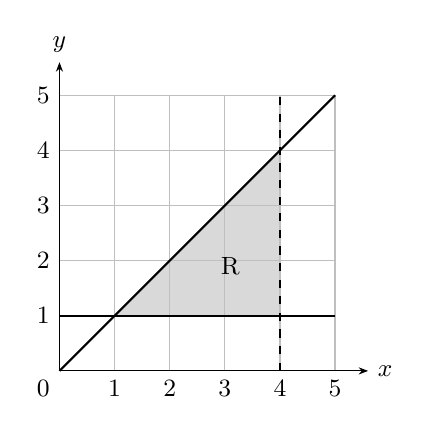
\begin{tikzpicture}[x=7mm,y=7mm,font=\small]
  \fill[black!15] (1,1) -- (4,1) -- (4,4) -- cycle;
  \draw[black!25,step={(1,1)}] (0,0) grid (5,5);
  \draw[-{Stealth[length=1.2mm]}] (0,0) -- (5.6,0) node[right] {$x$};
  \draw[-{Stealth[length=1.2mm]}] (0,0) -- (0,5.6) node[above] {$y$};
  \foreach \t in {1,...,5}{\node[below] at (\t,0) {\t}; \node[left] at (0,\t) {\t};}
  \node[below left] at (0,0) {0};
  \draw[thick] (0,1) -- (5,1);
  \draw[thick,dashed] (4,0) -- (4,5);
  \draw[thick] (0,0) -- (5,5);
  \node at (3.1,1.9) {R};
\end{tikzpicture}
\ealpara{Narysuj układ \ealkeytr{osi} z $x$ i $y$ od $-1$ do 5. Zacieniuj \ealkeytr{obszar}, w którym $x\ge0$, $y\ge1$ i $x+y\le4$. Ile \ealkeytr{punktów} o \ealkeytr{współrzędnych} będących \ealkeytr{liczbami całkowitymi nieujemnymi} znajduje się w tym \ealkeytr{obszarze}, łącznie z jego krawędziami?}{\q Draw a set of \ealkey{axes}, with $x$ and $y$ from $-1$ to 5. Shade the \ealkey{region} where $x\ge0$, $y\ge1$ and $x+y\le4$. How many \ealkey{points} with \ealkey{whole-number} \ealkey{coordinates} are in the \ealkey{region}, including its edges?}

% ----------------------------------------------------------------
\ealpara{Dzielenie przez \ealkeytr{liczbę ujemną}}{\topic{Dividing by a \ealkey{negative number}}}
\ealpara{\ealkeytr{Rozwiąż}\quad (a) $-2x>8$\qquad (b) $-5x\le-15$\\[2pt]
(c) $7-3x<1$}{\q \ealkey{Solve}\quad (a) $-2x>8$\qquad (b) $-5x\le-15$\\[2pt]
(c) $7-3x<1$}
\ealpara{Jo \ealkeytr{rozwiązuje} $10-2x>4$ i otrzymuje $x>3$. Sprawdź $x=4$ w $10-2x>4$ i wyjaśnij błąd Jo.}{\q Jo \ealkey{solves} $10-2x>4$ and gets $x>3$. Test $x=4$ in $10-2x>4$, and explain Jo's mistake.}

% ----------------------------------------------------------------
\ealpara{\ealkeytr{Rozwiązywanie} problemów}{\topic{Problem \ealkey{solving}}}
\ealpara{Znajdź wszystkie \ealkeytr{liczby całkowite}, które \ealkeytr{spełniają} zarówno $3x-1>5$, jak i $2x+3\le15$.}{\q Find all the \ealkey{integers} that \ealkey{satisfy} both $3x-1>5$ and $2x+3\le15$.}
\ealpara{Zapisz \ealkeytr{nierówność podwójną}, której \ealkeytr{rozwiązaniami} są dokładnie \ealkeytr{liczby całkowite} $-2$, $-1$, 0 i 1.}{\q Write a \ealkey{double inequality} whose \ealkey{integer} \ealkey{solutions} are exactly $-2$, $-1$, 0 and 1.}
\ealpara{Plan telefoniczny A kosztuje £10 miesięcznie plus 5p za każdą minutę rozmów. Plan B kosztuje £18 miesięcznie plus 1p za każdą minutę. Przy ilu minutach rozmów w miesiącu plan B jest tańszy?}{\q Phone plan A costs £10 a month, plus 5p for each minute of calls. Plan B costs £18 a month, plus 1p for each minute. For how many minutes of calls in a month is plan B cheaper?}

\end{multicols}

\end{document}